% ============================================================
%  Context-Dependent Precision Utility for Mixed-Precision
%  Object Detection -- ICASSP 2027 submission draft
%  Compile: pdflatex main.tex (twice) or latexmk -pdf main.tex
% ============================================================
\documentclass{article}
\usepackage{spconf,amsmath,amssymb,graphicx,booktabs,hyperref}
\usepackage{algorithm,algorithmic}
\usepackage{balance}
\usepackage[T1]{fontenc}
\hypersetup{hidelinks,hypertexnames=false,
  pdftitle={Context-Dependent Precision Utility for Mixed-Precision Object Detection},
  pdfauthor={Dongxu Liu}}
\def\BibTeX{{\rm B\kern-.05em{\sc i\kern-.025em b}\kern-.08em
    T\kern-.1667em\lower.7ex\hbox{E}\kern-.125emX}}

% Compact author block: drop the blank row after the name row (official
% fonts/margins unchanged; needed to keep the 4-page content limit).
\makeatletter
\def\name#1{\gdef\@name{{\em #1}}}
\def\@maketitle{\newpage
 \null
 \vskip 1em \begin{center}
 {\large \bf \@title \par} \vskip .75em {\large \lineskip .5em
\begin{tabular}[t]{c}\@name \\ \@address
 \end{tabular}\par} \end{center}
 \par
 \vskip 1em}
\makeatother

% Modest float/display spacing tightening (official margins and 10pt body
% unchanged); needed to keep the 4-page content limit with the full author block.
\setlength{\textfloatsep}{3pt plus 1pt minus 1pt}
\setlength{\floatsep}{3pt plus 1pt minus 1pt}
\setlength{\intextsep}{3pt plus 1pt minus 1pt}
\setlength{\abovedisplayskip}{3pt plus 1pt minus 1pt}
\setlength{\belowdisplayskip}{3pt plus 1pt minus 1pt}

\title{Context-Dependent Precision Utility for\\ Mixed-Precision Object Detection}

% ICASSP 2027 is NOT double-blind; keep author block.
\name{Dongxu Liu$^{1}$\sthanks{Corresponding author.}, Linhao Wang$^{2}$, Chenrui Zhu$^{3}$, Dongyang Liu$^{4}$}
\address{$^{1}$School of Artificial Intelligence, Jilin University, Changchun, China\\
$^{2}$College of Computer Science and Technology, Jilin University, Changchun, China\\
$^{3}$College of Software, Jilin University, Changchun, China\\
$^{4}$Yingcai Honors College, University of Electronic Science and Technology of China, Chengdu, China\\
{\footnotesize E-mail: liudx9924@mails.jlu.edu.cn, lhwang2124@mails.jlu.edu.cn, zhucr5525@mails.jlu.edu.cn, 2024310102018@std.uestc.edu.cn}}

\begin{document}

\maketitle
\vspace{-0.75em}

\begin{abstract}
Mixed-precision quantization (MPQ) is a key enabler for deploying object
detectors at the edge: assigning different bit-widths to different layers
trades accuracy for cost far more efficiently than uniform quantization.
The dominant recipe scores each layer's precision sensitivity
independently and allocates bits from these singleton scores. In this
paper we show, through controlled measurements on Mask R-CNN with a
Swin-T backbone, that this independence assumption breaks in detectors:
precision utility is context-dependent, with pairwise interactions at
$0.79\times$ the scale of singleton effects, $22.6$--$32.0\%$ ranking
reversals across five calibration seeds, and up to $3.6$ AP of
decision-level impact at equal budget. We then present a labels-free
allocation method that measures conditional marginal utility directly on
64 unlabeled images, stabilizes the search with an $\varepsilon$-tolerant
split-half criterion, and refines allocations with budget-neutral
pairwise exchanges; a sample-complexity analysis explains why 64 images
suffice. At matched parameter-weighted budgets on COCO, the method leads
at every practical budget (e.g., $+5.2$ AP over uniform-4 at $4.0$-bit
and $+1.8$ at $4.5$-bit) and transfers to a second backbone (Swin-S,
$+12.5$ at $4.5$-bit).
Code is available at \url{https://github.com/ldx825/Mixed-Precision-Object-Detection_ICASSP-2027}.
\end{abstract}

\begin{keywords}
mixed-precision quantization, object detection, bit allocation,
calibration, model compression
\end{keywords}

% ============================================================
\section{Introduction}
\label{sec:intro}
% ============================================================

Deploying object detectors at the edge requires quantization
\cite{jacob2018quant,gholami2022survey}, and
mixed-precision quantization (MPQ)---spending high precision only where
it matters---promises a better accuracy--cost trade-off than uniform
bit-widths. The dominant recipe is two-staged: (i) score the
``sensitivity'' of each parameter group (layer, block, or channel)
independently, once, at full precision or at a fixed reference state;
(ii) solve a budgeted allocation problem over these per-group scores
\cite{hawq,haq,bitsplit,flbq,lampq,blobq,regptq}. A silent assumption
underlies stage (i): that a group's contribution is an
\emph{intrinsic, context-free} property.

This paper shows that in object detection this assumption fails, and we
build an allocation method around its failure.

\smallskip
\noindent\textbf{(1) The problem: precision utility is context-dependent.}
  Using a controlled instrument---fake quantization of the 12 transformer
  blocks of a Swin-T backbone inside Mask R-CNN \cite{maskrcnn,swin}, with
a fully GT-free utility defined by agreement with the full-precision (FP)
teacher detector on 64 unlabeled images---we measure precision utility in
\emph{context}: the marginal value of repairing a block given that other
blocks are already repaired. Three findings emerge: pairwise interactions
average $0.79\times$ the size of singleton effects; conditional and
singleton rankings reverse on $22.6$--$32.0\%$ of within-context pairs
across five calibration seeds (Fig.~\ref{fig:reversal}); and at an
identical repair budget, decisions made from singleton rankings lose
$3.56$ AP with respect to conditional measurement (singleton top-4:
$41/495$; conditional: $11/495$, by exact enumeration).

\smallskip
\noindent\textbf{(2) The method: GT-free conditional allocation.}
We present a \emph{conditional} allocation method: it estimates marginal
utility in the current allocation context with the same instrument,
stabilizes noisy 64-image estimates with an $\varepsilon$-tolerant
split-half criterion over single upgrades and budget-neutral pairwise
exchanges, and selects among several starting allocations by full-64
utility. It requires no labels, no retraining, and only
$\sim\!10^{2}$--$10^{3}$ calibration forwards.

\smallskip
\noindent\textbf{(3) The results: best-or-tied at every budget, two backbones.}
At matched parameter-weighted budgets on COCO 5k \cite{coco}, the method
attains the best-or-tied deployable accuracy at every tested budget
(e.g., $+1.8$ over the strongest reimplemented prior at $4.5$-bit), with
the margins holding when the strongest baseline is granted the same
extended bit-level set. It transfers to a second backbone of a different
size (Swin-S, $+12.5$ at equal budget), and it comes with analyses that
explain \emph{why} it works: a sample-complexity account of why $64$
calibration images suffice, and a reversal-floor law that predicts the
measured reversal rate and yields a design criterion for when singleton
scoring is structurally unreliable.

% ============================================================
\section{Related Work}
\label{sec:related}
% ============================================================

\noindent\textbf{Post-training quantization and bit allocation.}
PTQ has matured from uniform rounding \cite{gptq,adaround,repqvit} and
learned step sizes \cite{jacob2018quant,esser2020lsq}
to mixed precision, where layers receive different bit-widths under a size or
bit budget \cite{haq,hawq,bitsplit,dong2020hawqv2,yao2021hawqv3},
including reconstruction-based \cite{nagel2021brecq,wei2022qdrop}
and activation-aware LLM objectives \cite{xiao2023smoothquant,lin2024awq}.
Most mixed-precision methods follow
the score-then-allocate template, which itself inherits the classical
sensitivity-pruning lineage \cite{lecun1990obd}: compute
a per-layer sensitivity---often
Hessian- or Fisher-based \cite{hawq,lampq}, sometimes
task-metric- or
regression-based \cite{regptq}---and then solve a budgeted program (DP,
ILP, or Lagrangian search) over these independent scores.

\smallskip
\noindent\textbf{Detector-specific quantization.}
Detector backbones have evolved from CNN detectors
\cite{ren2015faster} to transformer detectors
\cite{carion2020detr,zhu2021deformable} and ViT-style backbones
\cite{dosovitskiy2021vit}, with dedicated PTQ designs
\cite{li2022ptq4vit,liu2021qvit,lin2022fqvit}.
F-LBQ \cite{flbq} allocates transformer-layer bit-widths by minimizing
backbone-feature alteration (uniform quantization on heads; layer-wise
feature-space proxy). LampQ \cite{lampq} uses a type-aware Fisher-style
score with an ILP allocation and reports Mask R-CNN + Swin-T detection
results at 4-bit weight/activation. Reg-PTQ \cite{regptq} targets the
regression branch with a global reconstruction loss. These works share
the singleton-score premise; we instead measure \emph{conditional}
utility and show the singleton premise is quantitatively unreliable for
detector allocation decisions.

\smallskip
\noindent\textbf{Output-distortion objectives.}
BLOB-Q \cite{blobq} approximates global distortion by a second-order
expansion and, under a layer-uncorrelatedness assumption, decomposes it
into additive terms enabling DP allocation; it reports Mask R-CNN +
Swin-T/S detection at 4/5/6-bit. We test the
\emph{operational consequence} of additive decomposition: can
context-free contributions predict which block deserves extra precision
\emph{after} others changed? Our interaction and rank-reversal
measurements indicate they cannot (Sections~\ref{sec:mech},
\ref{sec:exp}), which motivates measuring marginals in context.

\smallskip
\noindent\textbf{Calibration without labels.}
Most quantization calibration uses unlabeled data
\cite{cai2020zeroq,krishnamoorthi2018}; what varies is the
quantity measured. Feature-space proxies \cite{flbq}, output-level
quadratic objectives \cite{blobq}, and gradient/Fisher statistics
\cite{lampq} can all be computed without labels. Ours also needs no
labels---only FP-teacher detections---but measures \emph{task-output
agreement in the current context} rather than a singleton proxy, with a
sample-size analysis (Sec.~\ref{sec:theory}).

\smallskip
\noindent\textbf{Reimplementation note.} Prior-art comparators are
labeled reimplementations/stand-ins (feature-MSE for F-LBQ-style,
additive output sensitivity for BLOB-Q-style, and a Fisher-style score
for LampQ-style); they share our quantizer, calibration set and budget
accounting, and are not the official pipelines.

% ============================================================
\section{Preliminaries}
\label{sec:prelim}
% ============================================================

\noindent\textbf{Model and quantization contract.}
We use the official Mask R-CNN with Swin-T (mmdetection 3.3.0) and its
released COCO checkpoint. FP bbox/mask AP is $42.65$/$39.28$ on val2017
(5k). The allocation units are the 12 Swin-T blocks; each block comprises
four weight groups $\{$qkv, proj, fc1, fc2$\}$, and every group receives
symmetric min-max per-tensor weight-only fake quantization at a bit-width
$b\in\{3,\ldots,8\}$ (the main sweep spans $\{4,\ldots,8\}$; the
$4.0$-bit regime additionally exploits level $3$, see
Sec.~\ref{sec:exp}); heads, LayerNorm, embeddings and biases remain FP.
Blocks differ $60\times$ in size ($0.11$--$7.1$M; Stage-3 dominates). The \emph{budget} of an allocation $\mathbf{b}$ is
the parameter-weighted average bit
$\bar{b}(\mathbf{b})=\sum_g n_g b_g / \sum_g n_g$, where $n_g$ is the
number of weights in group $g$. All methods compare at identical
$\bar{b}$.

\smallskip
\noindent\textbf{GT-free utility.}
Let the FP model be the teacher. For a quantized state with repaired set
$S$ (blocks in $S$ at 8-bit, others at the base $\bar{b}$ configuration),
run the standard test pipeline on a fixed unlabeled calibration set (64
COCO train images by default) and match teacher and student detections
per image and class (greedy by teacher score, IoU $\geq 0.5$, teacher
score $\geq 0.3$). Define
\begin{equation}
U(S) \;=\; -\,\mathrm{score\_drop}(S)
\;=\;-\,\overline{\big(s^{\mathrm{FP}} - s^{\mathrm{q}}\big)}_{\text{matched pairs}},
\label{eq:utility}
\end{equation}
the negative mean score gap over matched teacher--student pairs (pooled
over images; boxes only; no ground truth anywhere). The
\emph{conditional marginal utility} of repairing block $i$ given context
$S$ is
$\Delta(i\mid S) = U(S\cup\{i\}) - U(S)$,
and the pairwise interaction is
$I_{ij} = U(\{i,j\}) - U(\{i\}) - U(\{j\}) + U(\varnothing)$
(centered at the base state; without the $+U(\varnothing)$ term the raw
interaction is dominated by the offset $|U(\varnothing)|$ and is
uninformative).
$U$ is measured, not modeled: no Hessian, no proxy features, no labels.

% ============================================================
\section{Detector Precision Utility is Context-Dependent}
\label{sec:mech}
% ============================================================

\noindent\textbf{Non-additive interactions.}
We measured all $\binom{12}{2}=66$ pairwise interactions on a 6-bit base
(all blocks at 6-bit; $U(\varnothing)$ has score\_drop $0.0298$).
Table~\ref{tab:interaction} summarizes: the average absolute centered
interaction is $0.00135$ versus mean $|\Delta(i\mid\varnothing)|=0.00171$,
a ratio of $0.79$.
Extremes are instructive: \texttt{BLK2.3}$+$\texttt{BLK2.5} are nearly
useless alone yet interact by $+0.0060$, while two of the best singletons
(\texttt{BLK2.0}/\texttt{BLK2.2}) underperform their sum by $-0.0047$.

\begin{table}[t]
\centering
\small
\caption{Pairwise interactions, 6-bit base (calib-64, GT-free).}
\label{tab:interaction}
\begin{tabular}{lr}
\toprule
statistic & value \\
\midrule
mean $I_{ij}$ & $+0.0005$ \\
std $I_{ij}$ & $0.0017$ \\
range & $[-0.0047, +0.0060]$ \\
mean $|I_{ij}|$ & $0.00135$ \\
mean $|\Delta(i\mid\varnothing)|$ & $0.00171$ \\
ratio & $0.79$ \\
\bottomrule
\end{tabular}
\end{table}

\begin{figure}[t]
\centering
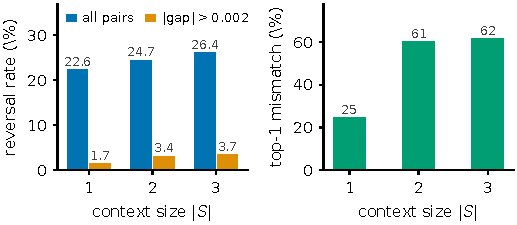
\includegraphics[width=0.98\linewidth]{figures/fig1_reversal.pdf}
\caption{Singleton-vs-conditional ranking under growing context:
(a)~pairwise order reversal rate (all pairs vs.\ large-gap pairs,
$|{\rm gap}|>0.002$); (b)~top-1 mismatch rate.}
\label{fig:reversal}
\end{figure}

\noindent\textbf{Rank reversal.}
If interactions were small or homogeneous, singleton rankings would still
be usable. They are not: comparing, for every context $S$, the conditional
ranking $\Delta(i\mid S)$ against the singleton ranking
$\Delta(i\mid\varnothing)$ over the remaining candidates, $22.6\%$,
$24.7\%$, $26.4\%$ of pairwise orders reverse at $|S|{=}1,2,3$
(Fig.~\ref{fig:reversal}; $12/66/220$ contexts, top-1 mismatch
$25/61/62\%$). Reversals are mostly moderate in size, but the largest
reversals change decisions: in context
$S=\{\texttt{BLK2.5},\texttt{BLK3.0}\}$ conditional measurement prefers
\texttt{BLK2.3} over the singleton-favored \texttt{BLK2.4}, a $+0.0070$
utility swing ($\approx 4\times$ the mean singleton effect).

\smallskip
\noindent\textbf{Five-seed replication.}
Four additional 64-image pools give reversal rates of
$22.6$--$32.0\%$ (all $\geq 20\%$) and interaction-to-singleton ratios
of $0.50$--$1.12$ (mean $0.76$); per-pair values are seed-dependent, so
we report distribution-level statements, which all replicate.

\smallskip
\noindent\textbf{Decision impact.}
Utility-level differences translate to decisions. At an equal repair
budget (4 of 12 blocks at 8-bit, 4-bit base), selecting blocks by
singleton rankings of the same instrument gives $31.39$ AP---about
chance-level among repair sets ($31.07$)---while conditional measurement
gives $34.95$ ($+3.56$), and the oracle repair set gives $35.32$. Exact
enumeration of all $\binom{12}{4}=495$ sets confirms the ordering
(top-4: $41/495$ vs.\ $11/495$); predicted and
measured gains correlate at Spearman $0.72$--$1.00$ (legal signals)
vs.\ $-0.16$--$0.60$ (feature proxy).

% ============================================================
\section{Method: GT-Free Conditional Allocation}
\label{sec:method}
% ============================================================

The method has four components; Algorithm~\ref{alg:method} summarizes
the complete pipeline.

\begin{algorithm}[t]
\caption{GT-free conditional allocation at budget $\bar b$.}
\label{alg:method}
\begin{algorithmic}[1]
\REQUIRE FP teacher; $N$ blocks with precision ladder $\mathcal L$;
budget $\bar b$; calibration set $\mathcal C$ ($n$ unlabeled images);
starts $\mathcal S_0$; tolerance $\varepsilon$
\ENSURE deployed allocation $\mathbf b^{\star}$
\STATE $\mathrm{Util}(\mathbf b)$: run the test pipeline on $\mathcal C$
with $\mathbf b$; match teacher--student detections per image and class
(greedy by score, at fixed matching thresholds); return
$-\mathrm{score\_drop}$ (Eq.~\eqref{eq:utility})
\STATE \textbf{Phase 1 (conditional greedy).} $\mathbf b \leftarrow \mathbf b_{\mathrm{base}}$
\WHILE{a feasible single-level upgrade fits the residual budget}
\STATE $i^{\star} \leftarrow \arg\max_i\,
[\mathrm{Util}(\mathbf b{+}\mathbf e_i)-\mathrm{Util}(\mathbf b)]/n_i$
\COMMENT{$\mathbf e_i$ upgrades block $i$; re-measured in context}
\STATE $\mathbf b \leftarrow \mathbf b + \mathbf e_{i^{\star}}$;
\textbf{append} $\mathbf b$ to $\mathcal S_0$
\ENDWHILE
\STATE \textbf{Phase 2 ($\varepsilon$-tolerant refinement), per start $\mathbf b_s \in \mathcal S_0$:}
\REPEAT
\STATE split $\mathcal C$ into halves $A,B$; for each move $m$ in the
neighborhood (single-level swaps; budget-neutral pair exchanges, one level
up and one down) compute per-half score-gap changes $d_A(m),d_B(m)$
\STATE accept the best $m$ with $d_A{+}d_B>0$ and
$\min(d_A,d_B)\geq-\varepsilon$ (Eq.~\eqref{eq:eps});
$\mathbf b_s \leftarrow \mathbf b_s{+}m$
\UNTIL{no move accepted}
\STATE \textbf{Phase 3 (selection).} \textbf{return}
$\mathbf b^{\star} \leftarrow \arg\max_{\mathbf b_s \in \mathcal S_0}
\mathrm{Util}(\mathbf b_s)$ \COMMENT{full-64 utility; no labels, no 5k}
\end{algorithmic}
\end{algorithm}

\smallskip
\noindent\textbf{Conditional greedy.}
From the all-4-bit base, repeatedly perform the feasible single-level
upgrade maximizing gain-per-cost $\Delta(i\mid S)/n_i$
(Eq.~\eqref{eq:utility}), re-measuring in the new context after each
commit; stop when no upgrade fits the residual budget. Scores are
\emph{measured in the actual context in which the block will operate},
unlike singleton scores computed once at a fixed reference.

\smallskip
\noindent\textbf{$\varepsilon$-tolerant refinement.}
64-image measurements are noisy (cross-seed std $0.0016$, comparable to
typical swap effects, Sec.~\ref{sec:theory}). We split the 64 images into
two halves and accept a move iff
\begin{equation}
d_A + d_B > 0
\quad\text{and}\quad
\min(d_A, d_B) \geq -\varepsilon,
\qquad \varepsilon = 10^{-3},
\label{eq:eps}
\end{equation}
over a neighborhood of single-block $\pm1$ swaps and budget-neutral
pairwise exchanges $(i{:}+1, j{:}-1)$ at constant $\bar b$; iterate to a
fixed point.

\smallskip
\noindent\textbf{Multi-start and cost.}
We select among several starts (conditional greedy plus strong
baseline-produced allocations) by full-64 utility---no ground truth and
no 5k data enter the search. Per budget the pipeline uses
  $\sim\!10^3$--$10^4$ detector forwards ($\sim$400 greedy, $\sim$600--$900$

% ============================================================
\section{Sample-Complexity Analysis}
\label{sec:theory}
% ============================================================

The method ranks candidates and accepts moves by comparing
estimated utilities $\hat\mu_a = n^{-1}\sum_k Z_a(x_k)$, where $Z_a(x)$
is the bounded per-image utility contribution of move $a$
($|Z_a|\leq 1$). Two standard consequences link the calibration size
$n$ to allocation reliability.

\smallskip
\noindent\textbf{(T1) Correct comparisons.}
Let there be $M$ candidate moves per round and $R$ rounds
($M\!\leq\!150$, $R\!\leq\!8$ in our setting). By Hoeffding's inequality
\cite{hoe} and a union bound, if the comparison margin between the best
and second-best move is $\Delta\mu$ (in per-image mean units), then
\begin{equation}
n \;\geq\; \frac{2}{\Delta\mu^{2}}\,
\log\!\Big(\frac{2MR}{\delta}\Big),
\label{eq:t1}
\end{equation}
suffices for the measured search trajectory to match the
exact-utility trajectory with probability $\geq 1-\delta$.

\smallskip
\noindent\textbf{(T2) $\varepsilon$-optimal acceptance.}
The acceptance rule Eq.~\eqref{eq:eps} only asks for moves that are
$\varepsilon$-close to optimal; the standard relaxation gives
\begin{equation}
n \;\geq\; \frac{2}{\varepsilon^{2}}\,
\log\!\Big(\frac{MR}{\delta}\Big),
\label{eq:t2}
\end{equation}
so tolerance and sample size trade off quadratically---the
methodological reason a small $\varepsilon$ paired with 64 images is a
principled operating point rather than a heuristic.

\smallskip
\noindent\textbf{(T3) Interaction-conditioned reversal floor.}
Two candidates $a,b$ flip order between singleton and context-$S$
evaluation iff the interaction sum
$X_S=\sum_{j\in S}(I_{aj}-I_{bj})$ opposes and exceeds the singleton gap
$D=\Delta_a(\varnothing)-\Delta_b(\varnothing)$. Under symmetric
independent errors the expected reversal rate is
\begin{equation}
R \;=\; \tfrac12\, \mathrm{P}\big(|X_S| > |D|\big).
\label{eq:t3}
\end{equation}
On our measured tables Eq.~\eqref{eq:t3} predicts $R=22.1\%$ at
$|S|{=}1$; exact enumeration with the measured $U$ values gives
$22.58\%$, equal to the independent Exp31 measurement. Design criterion: $R<5\%$ needs
$\rho=\overline{|I|}\,/\,\overline{|\Delta|}$ below $0.134$---detectors
  measure $0.76$: no calibration budget repairs a singleton design.

\smallskip
\noindent\textbf{Theory meets measurement.}
At $n{=}64$ the cross-seed noise ($0.0016$) is $0.75\times$ the mean
effect ($0.0021$) and shrinks as $1/\sqrt n$; top-1 selection
stabilizes at $64$--$128$ images, matching the $(1/\Delta\mu^{2})$
scaling of Eq.~\eqref{eq:t1}.

\smallskip
\noindent\textbf{Scope.}
The analysis is at the level of the \emph{proxy utility} actually
measured (proxy-to-AP is empirical, Spearman $0.72$--$1.00$); the
guarantee is that noise does not misdirect the local search---not
global optimality.

% ============================================================
\section{Experiments}
\label{sec:exp}
% ============================================================

\noindent\textbf{Setup.}
Full COCO val2017 (5k) bbox AP with pycocotools under the
Sec.~\ref{sec:prelim} contract. Baselines: \textbf{uniform};
\textbf{F-LBQ-reimpl} (feature-MSE greedy); \textbf{BLOBQ-reimpl}
(output-damage curves); \textbf{LampQ-style} (Fisher-style);
\textbf{static-OUT}; \textbf{oracle-approx} (reference).

\begin{table}[t]
\centering
\small
\setlength{\tabcolsep}{3.5pt}
\caption{COCO 5k bbox AP at matched parameter-weighted budgets ($\bar b$);
bold = best deployable per budget. FP $=42.65$. F-LBQ/BLOBQ/LampQ are
  reimplementations; s-OUT $=$ static-OUT. ``Ours'' uses the extended level
  set (level $3$); under the same extended contract the strongest baseline
  also reaches $22.65$ at $4.0$-bit and $35.72$ at $4.5$-bit (cf.\ fairness
  notes).}
\label{tab:main}
\begin{tabular}{lcccccc}
\toprule
$\bar b$ & unif. & F-LBQ & BLOBQ & LampQ & s-OUT & \textbf{Ours} \\
\midrule
4.0 & 17.41 & 17.41 & 17.41 & 17.41 & 17.41 & \textbf{22.65} \\
4.5 & 17.41 & 35.03 & 34.74 & 32.83 & 33.84 & \textbf{36.80} \\
5.0 & 39.57 & 37.93 & 39.87 & 39.57 & 39.57 & \textbf{39.91} \\
5.5 & 39.57 & 40.28 & 40.92 & 40.94 & 41.18 & \textbf{41.62} \\
6.0 & 41.96 & 41.84 & 41.94 & 41.96 & 41.96 & \textbf{42.01} \\
\bottomrule
\end{tabular}
% Final numbers; Ours = pipeline output (conditional greedy + accepted
% refinements; the multi-start set includes baseline-produced allocations,
% and the deployed configuration is selected by 64-image utility alone).
\end{table}

\noindent\textbf{Main results.}
Our method attains the best-or-tied deployable AP at every tested
budget: $+5.24$ over uniform-4 at $4.0$-bit (extended level set;
ties the strongest fair-contract baseline at $22.65$), $+1.77$ at $4.5$,
$+0.04$ at $5.0$, $+0.44$ at $5.5$,
and $+0.05$ at $6.0$ (a completion step spends the leftover $0.05$ bit).
The cross-strategy spread is $3.9$ AP at $4.5$-bit ($32.83$--$36.80$),
collapsing to $0.12$ AP at $6.0$-bit.

\smallskip
\noindent\textbf{What wins.}
Winning allocations pile precision on \emph{shallow, cheap} blocks
(stages 0--1, 0.1--0.4M weights; up to 8-bit) while the dominating
stage-3 blocks receive \emph{differentiated} precision: at $4.5$-bit one
parameter-neutral Stage-3 swap ($4\!\to\!3$ next to $4\!\to\!5$) is worth
$+1.21$ AP. Reallocation---not singleton ranking---separates the methods:
uniform-4 scores $17.41$ AP, while the same budget reallocated reaches
$36.80$.

\smallskip
\noindent\textbf{Ablation: search design.}
At $4.5$-bit: strict split-half validation rejects true improvements
(full-chain: $33.84$, $-1.75$); the $\varepsilon$-tolerant criterion plus
pair exchanges (incl.\ level-3 moves) reaches $36.80$.

\smallskip
\noindent\textbf{Second backbone.}
On Mask R-CNN + Swin-S ($24$ blocks, same contract; FP $=48.18$), the
same procedure reaches $44.74$ AP at the $4.5$-bit budget versus $32.22$
for uniform-4---not Swin-T specific.

\smallskip
\noindent\textbf{Calibration-size behavior.}
Five 64-image pools give cross-seed top-1 agreement of
$80\%$/$100\%$ at $n{=}64$/$n\!\geq\!128$ (Eq.~\eqref{eq:t1}).

\smallskip
\noindent\textbf{Fairness notes.} All comparators share our quantizer
(weight-only) and budget; prior published numbers use weights and
activations together and are therefore not directly comparable to ours
(bridging the two is follow-up work).
Under the fair extended contract (level $3$ granted to all), our deployed
outputs lead at $4.5$--$6.0$ ($+1.08$, $+0.04$, $+0.44$, $+0.05$) and tie
the strongest baseline at $4.0$ ($22.65$); the feature-MSE baseline
collapses to $25.48$ at $4.5$, exposing the $3$-bit blind spot of
singleton signals.

% ============================================================
\enlargethispage{5\baselineskip}
\section{Conclusion}
\label{sec:concl}
% ============================================================

\looseness=-1
Singleton scoring assumes each layer's precision sensitivity is
fixed. On a Mask R-CNN + Swin-T detector it breaks:
precision utility is context-dependent---pairwise interactions match
singleton effects ($0.79\times$), $22.6$--$32.0\%$ of within-context
rankings reverse, and the errors cost measurable AP ($-3.56$). We
address the failure with a GT-free method that measures conditional
marginal utility on unlabeled images, using an $\varepsilon$-tolerant
split-half search and budget-neutral exchanges; it leads at every
tested budget and transfers to Swin-S. Limitations: weight-only, single family, proxy theory; future
work: weight-and-activation alignment and broader detector families.


\balance
\clearpage
% Official spconf.sty bibliography definition, with the inter-item separation
% slightly tightened so that all 33 refs fill (and fit) the final page at the
% body font size (10pt, per the ICASSP requirement of >= 9pt).
\makeatletter
\def\thebibliography#1{\section{References}\list
 {[\arabic{enumi}]}{\settowidth\labelwidth{[#1]}\leftmargin\labelwidth
 \advance\leftmargin\labelsep
 \itemsep 3.1pt plus 0.5pt minus 1.2pt
 \usecounter{enumi}}
 \def\newblock{\hskip .11em plus .33em minus .07em}
 \sloppy\clubpenalty4000\widowpenalty4000
 \sfcode`\.=1000\relax}
\makeatother
\bibliographystyle{IEEEbib}
\bibliography{refs}
\iffalse  % legacy manual bibliography (superseded by the official BibTeX flow above)
\begin{thebibliography}{99}
\bibitem{maskrcnn} K.~He, G.~Gkioxari, P.~Doll\'ar, and R.~Girshick,
  ``Mask R-CNN,'' in \textit{Proc. ICCV}, 2017.
\bibitem{swin} Z.~Liu \textit{et al.}, ``Swin Transformer: Hierarchical
  vision transformer using shifted windows,'' in \textit{Proc. ICCV}, 2021.
\bibitem{coco} T.-Y.~Lin \textit{et al.}, ``Microsoft COCO: Common objects
  in context,'' in \textit{Proc. ECCV}, 2014.
\bibitem{gptq} E.~Frantar \textit{et al.}, ``GPTQ: Accurate post-training
  quantization for generative pre-trained transformers,''
  in \textit{Proc. ICLR}, 2023.
\bibitem{hawq} Z.~Dong \textit{et al.}, ``HAWQ: Hessian aware quantization
  of neural networks with mixed-precision,'' in \textit{Proc. ICCV}, 2019.
\bibitem{haq} K.~Wang \textit{et al.}, ``HAQ: Hardware-aware automated
  quantization with mixed precision,'' in \textit{Proc. CVPR}, 2019.
\bibitem{bitsplit} P.~Wang \textit{et al.}, ``Bit-split and stitching:
  Efficient bitwidth search for practical mixed precision neural network,''
  arXiv:2003.07577, 2020.
\bibitem{flbq} \textit{[F-LBQ]} ``Feature-preserving layer-wise mixed
  precision quantization,'' in \textit{Proc. ICASSP}, 2026.
\bibitem{blobq} \textit{[BLOB-Q]} ``Global optimization of model distortion
  for layer-wise bit allocation,'' in \textit{Proc. ECCV}, 2026.
\bibitem{lampq} \textit{[LampQ]} ``Layer-wise mixed precision quantization
  for vision transformers,'' in \textit{Proc. AAAI}, 2026.
\bibitem{regptq} S.~Chen \textit{et al.}, ``Reg-PTQ: Regression-specialized
  post-training quantization for object detection,'' in \textit{Proc.
  CVPR}, 2024.
\bibitem{li2022ptq4vit} Y.~Li \textit{et al.}, ``PTQ4ViT: Post-training
  quantization for vision transformers with twin uniform quantization,'' in
  \textit{Proc. ECCV}, 2022.
\bibitem{repqvit} Z.~Li \textit{et al.}, ``RepQ-ViT: Scale reparameterization
  for post-training quantization of vision transformers,''
  in \textit{Proc. ICCV}, 2023.
\bibitem{adaround} M.~Nagel \textit{et al.}, ``Up or down? Adaptive
  rounding for post-training quantization,'' in \textit{Proc. ICML}, 2020.
\bibitem{jacob2018quant} B.~Jacob \textit{et al.}, ``Quantization and
  training of neural networks for efficient integer-arithmetic-only
  inference,'' in \textit{Proc. CVPR}, 2018.
\bibitem{esser2020lsq} S.~R. Esser \textit{et al.}, ``Learned step size
  quantization,'' in \textit{Proc. ICLR}, 2020.
\bibitem{krishnamoorthi2018} R.~Krishnamoorthi, ``Quantizing deep
  convolutional networks for efficient inference: A whitepaper,''
  arXiv:1806.08342, 2018.
\bibitem{gholami2022survey} A.~Gholami \textit{et al.}, ``A survey of
  quantization methods for efficient neural network inference,'' in
  \textit{Low-Power Computer Vision}, Chapman and Hall/CRC, 2022.
\bibitem{nagel2021brecq} M.~Nagel \textit{et al.}, ``BRECQ: Pushing the
  limit of post-training quantization by block reconstruction,'' in
  \textit{Proc. ICLR}, 2021.
\bibitem{wei2022qdrop} X.~Wei \textit{et al.}, ``QDrop: Randomly dropping
  quantization for extremely low-bit post-training quantization,'' in
  \textit{Proc. ICLR}, 2022.
\bibitem{dong2020hawqv2} Z.~Dong \textit{et al.}, ``HAWQ-V2: Hessian
  aware trace-weighted quantization of neural networks,'' in \textit{Proc.
  NeurIPS}, 2020.
\bibitem{yao2021hawqv3} Z.~Yao \textit{et al.}, ``HAWQ-V3: Dyadic neural
  network quantization,'' in \textit{Proc. ICML}, 2021.
\bibitem{liu2021qvit} Z.~Liu \textit{et al.}, ``Post-training quantization
  for vision transformer,'' in \textit{Proc. NeurIPS}, 2021.
\bibitem{lin2022fqvit} Y.~Lin \textit{et al.}, ``FQ-ViT: Post-training
  quantization for fully quantized vision transformer,'' in \textit{Proc.
  IJCAI}, 2022.
\bibitem{carion2020detr} N.~Carion \textit{et al.}, ``End-to-end object
  detection with transformers,'' in \textit{Proc. ECCV}, 2020.
\bibitem{zhu2021deformable} X.~Zhu \textit{et al.}, ``Deformable DETR:
  Deformable transformers for end-to-end object detection,'' in
  \textit{Proc. ICLR}, 2021.
\bibitem{ren2015faster} S.~Ren \textit{et al.}, ``Faster R-CNN: Towards
  real-time object detection with region proposal networks,'' in
  \textit{Proc. NeurIPS}, 2015.
\bibitem{xiao2023smoothquant} G.~Xiao \textit{et al.}, ``SmoothQuant:
  Accurate and efficient post-training quantization for large language
  models,'' in \textit{Proc. ICML}, 2023.
\bibitem{lin2024awq} J.~Lin \textit{et al.}, ``AWQ: Activation-aware
  weight quantization for on-device LLM compression and acceleration,'' in
  \textit{Proc. MLSys}, 2024.
\bibitem{dosovitskiy2021vit} A.~Dosovitskiy \textit{et al.}, ``An image
  is worth 16x16 words: Transformers for image recognition at scale,'' in
  \textit{Proc. ICLR}, 2021.
\bibitem{lecun1990obd} Y.~LeCun, J.~S. Denker, and S.~A. Solla, ``Optimal
  brain damage,'' in \textit{Proc. NeurIPS}, 1989.
\bibitem{cai2020zeroq} Y.~Cai \textit{et al.}, ``ZeroQ: A novel zero shot
  quantization framework,'' in \textit{Proc. CVPR}, 2020.
\bibitem{hoe} W.~Hoeffding, ``Probability inequalities for sums of bounded
  random variables,'' \textit{J. Amer. Statist. Assoc.}, vol.~58, no.~301,
  1963.
\end{thebibliography}
\fi

\end{document}
